\documentclass[12pt]{article}

\usepackage{graphicx}
\usepackage{amsmath}
\usepackage{amsfonts}
\usepackage{amssymb}
\usepackage{subcaption}
\usepackage{pdfpages}

\def\td{\mathbf{t}}   % response-threshold value

\begin{document}
\includepdf[pages={-}]{nature-text.pdf}

\newpage
\subsection*{Figures}

\begin{figure*}[ht!]
    \centering\begin{subfigure}[t]{0.5\textwidth}
        \centering
        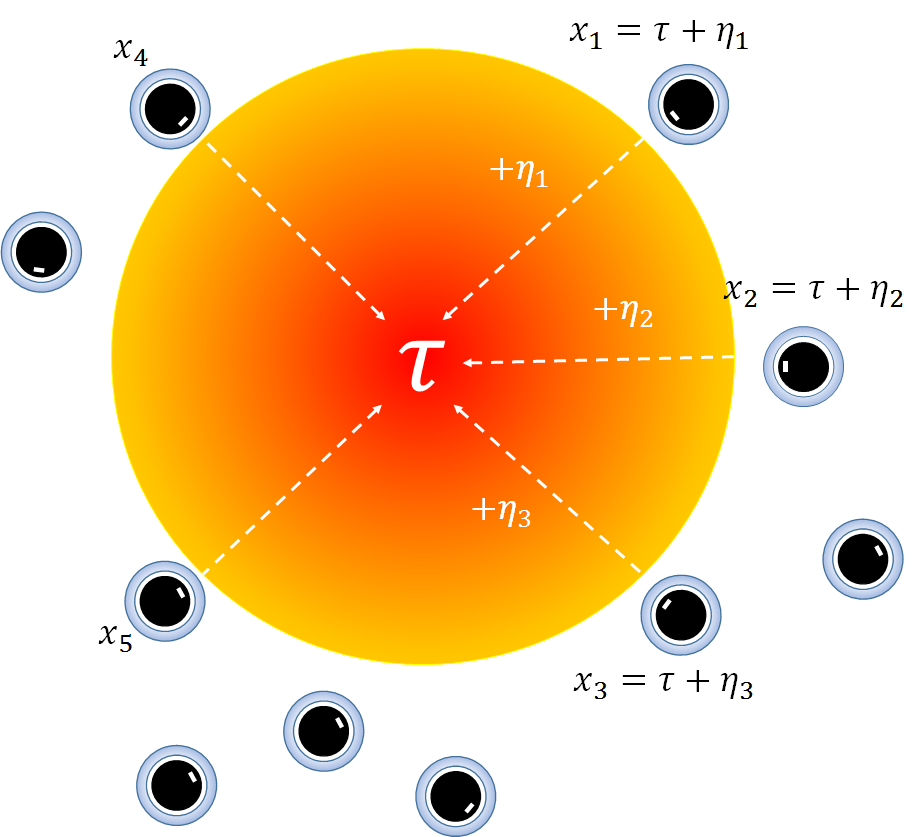
\includegraphics[width=1\textwidth]{figures/firefighting.png}
        \caption{}
    \end{subfigure}%
    ~ 
    \begin{subfigure}[t]{0.5\textwidth}
        \centering
        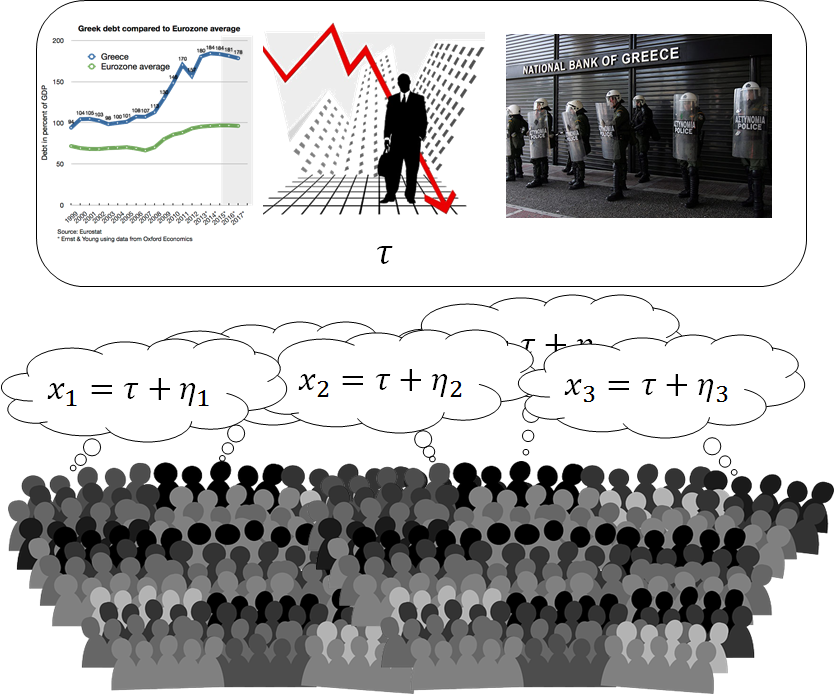
\includegraphics[width=1\textwidth]{figures/bankrun.png}
        \caption{}
    \end{subfigure}
    \begin{subfigure}[t]{1\textwidth}
        \centering
        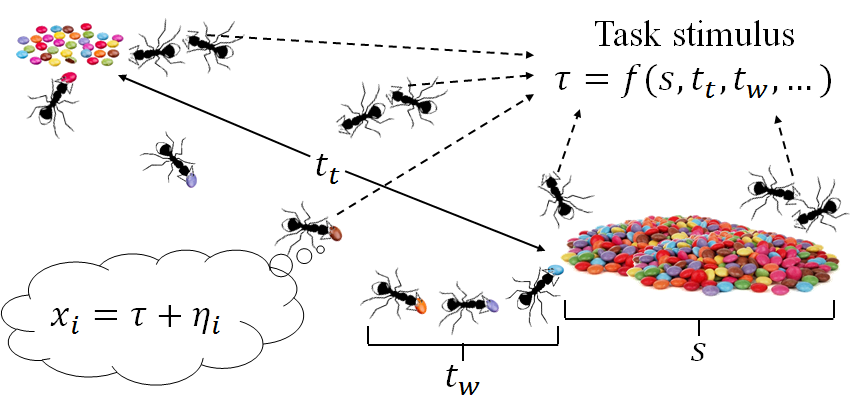
\includegraphics[width=1\textwidth]{figures/foraging.png}
        \caption{}
    \end{subfigure}    
    \caption{Caption place holder}    
\end{figure*}

%\begin{figure}[!ht]
%	\centering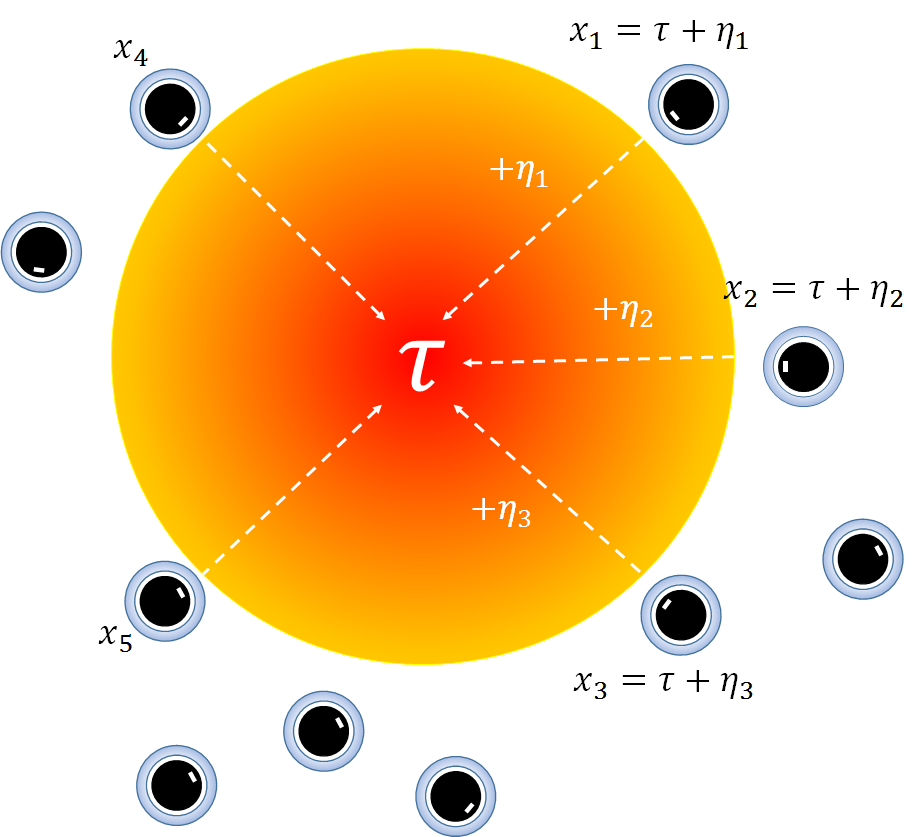
\includegraphics[width=\columnwidth]{figures/firefighting.png}
%	\centering\caption{A multi-agent fire fighting scenario set up as a global game. Each player's imperfect estimate of the task is represented by $x_i$, a sum of the global magnitude parameter-$\tau$ and noisy sensor measurements-$\eta_i$.}\vspace{-10px}
%\end{figure}
%
%\newpage
%\begin{figure}[!ht]
%	\centering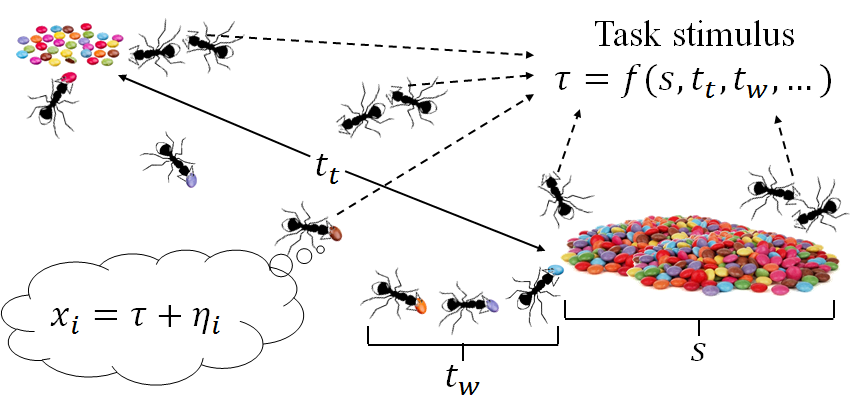
\includegraphics[width=\columnwidth]{figures/foraging.png}
%	\centering\caption{An ant foraging scenario presented as a global game with concurrent benefit. Each ant decides whether or not to participate in the food collecting task based on a number of environmental cues such as the travel time $t_t$ from the colony to the food source, the wait time in queue to drop off the collected food $t_w$, and the perceived amount of food already stored at the colony $s$. Inherent inaccuracies in measuring these variables are represented as a noise term $\eta_i$ in the agent’s perceived estimate of the global stimulus $\tau$.
%}\label{fig:thm2fig}
%\end{figure}
%
%\newpage
%\begin{figure}[!ht]
%	\centering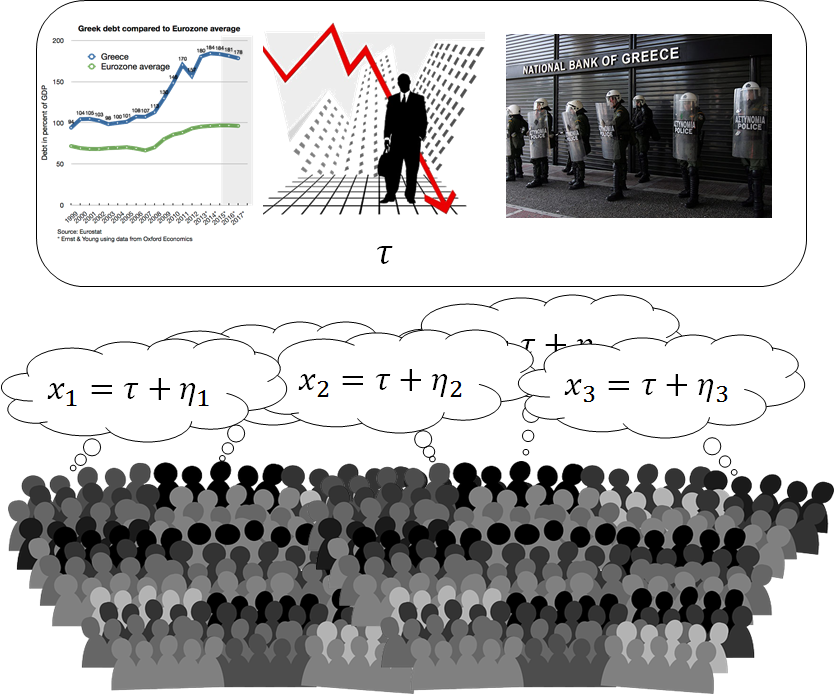
\includegraphics[width=\columnwidth]{figures/bankrun.png}
%	\centering\caption{A bank run scenario presented as a global game with concurrent benefit. As seen in Greece recently, a bank run can result from a complex combination of economic factors that are indirectly perceived by the populous as a common global signal $\tau$. Each individual has a noisy ($\eta_i$) mental estimate of $\tau$, labeled $x_i$, that represents their level of trust in the nation's economy. If this level of trust crosses an individually set threshold for enough of the populous a bank run occurs.
%}\label{fig:thm2fig}
%\end{figure}

\newpage
\begin{figure}[!ht]
	\centering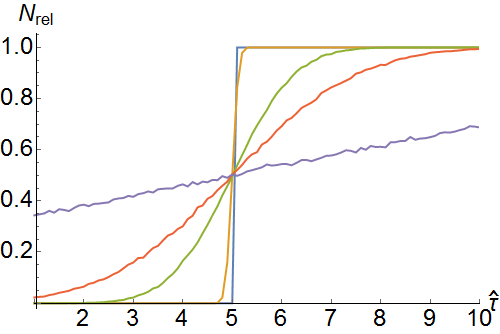
\includegraphics[width=\columnwidth]{figures/thm2fig.png}
	\centering\caption{Visualization of Theorem~2 as $N_{rel}$ estimates $\Phi(\cdot)$. The plot was generated by running Eqn.~1 10,000 times for each point in $\hat{\tau} = 1$ to $10$ in increments of $0.1$. $n = 10$, $\td = 5$ and $x_i = \hat{\tau} + \eta_i$ ($\eta_i \sim\mathcal{N}(0, \sigma^2)$). Each curve in the plot is generated by sweeping $\sigma^2 = \{0, 0.1, 1, 2, 10\}$, with $\sigma^2 = 0$ being a step-function and $\sigma^2 = 10$ having the \emph{flattest} slope.}\label{fig:thm2fig}
\end{figure}
\end{document}